\chapter{Special relativistic hydrodynamics}
\label{c:special-relativistic-hydrodynamics}
%\label{Relativistic Hydrodynamic Equations}
\section{Relativistic hydrodynamics}
\label{Relativistic Hydrodynamics}
Mass and energy-momentum conservation laws of a special relativistic ideal fluid follow
\begin{subequations}
\label{eq:conservation laws}
\begin{align}
&\partial_{\nu}\left(\rho U^{\nu}\right)=0, \label{eq:number conservation}\\
&\partial_{\nu}T^{\mu \nu} = 0, \label{eq:energy conservation}
\end{align}
\end{subequations}
where
\begin{equation}
T^{\mu \nu} = \rho h U^{\mu} U^{\nu}/c^2 + p \eta^{\mu \nu}.
\end{equation}
$\rho$ and $p$ are the proper mass density and the pressure, $U^\mu$ the four-velocity, $\eta^{\mu \nu}$ the metric tensor of Minkowski space, and $c$ the speed of light. $h$ is the specific enthalpy, related to the specific thermal energy $\epsilon$ by
\begin{equation}
  h=c^2+\epsilon +\frac{p}{\rho}.
  \label{eq:eos}
\end{equation}

An equation of state, $h\left(\rho, p\right)$, is required to close \Cref{eq:conservation laws} and will be discussed in Section \ref{EoS}.
Throughout this paper, lower-case Greek indices run from 0 to 3, Latin ones from 1 to 3, and the Einstein summation convention is used, except when stated otherwise.

\Cref{eq:conservation laws} can be rewritten into a convenient conservative form for numerical integration:
\begin{subequations}
  \label{conservative form}
  \begin{align}
   &\partial_{t} D+\partial_{j} \left(DU^{j}/\gamma\right)=0,\label{D evolution}\\
   &\partial_{t}M^{i}+\partial_{j} \left(M^{i}U^{j}/\gamma+p\delta^{ij}\right)=0,\label{M evolution}\\
   &\partial_t E+\partial_j  \left(M^{j}c^2\right)=0, \label{E evoltion}
  \end{align}
\end{subequations}
where $\gamma$ is the Lorentz factor, and $\delta^{ij}$ is the Kronecker delta notation.

The five conserved quantities $D$, $M^{i}$, and $E$ are the mass density, the momentum densities, and the total energy density, respectively. All conserved variables are related to primitive variables ($\rho, U^{i}, p$) through
\begin{subequations}
  \begin{align}
    &D=\rho\gamma,\label{density}\\
    &M^{i}=Dh U^{i} /c^2,\label{momentum}\\
    &E=D h\gamma-p. \label{definition of reduced energy}
  \end{align}
  \label{relation between prim and cons}
\end{subequations}
Nevertheless, \cite{NR_Limit} suggest evolving the reduced energy density,
\begin{equation}
\tilde{E} \coloneqq E-Dc^2, \label{ETilde}
\end{equation}
instead of the total energy density; otherwise, extraction of a tiny thermal energy for a cold gas from the total energy will lead to catastrophic cancellation. An intuitive approach is to subtract \Cref{D evolution} from \Cref{E evoltion} so that we can obtain a new energy equation. However, the new energy flux, $\left(M^{j}-DU^{j}/\gamma\right)c^2$, also suffers from catastrophic cancellation in the NR limit. An appropriate new energy flux avoiding such a problem is $(\tilde{E}+p)U^{j}/\gamma$, which is mathematically equivalent to $\left(M^{j}-DU^{j}/\gamma\right)c^2$. The reduced energy equation for numerical integration can thus be cast into
\begin{equation}
    \partial_t \tilde{E}+\partial_j \left[\left(\tilde{E}+p\right)U^{j}/\gamma\right]=0,
    \label{ETilde evolution}
\end{equation}
which is to replace \Cref{E evoltion}.

%\Cref{conservative form,relation between prim and cons} clearly show that we have taken advantage of explicitly adopting four-velocities ($U^{i}$) instead of three-velocities ($v^i=U^i/\gamma$) for numerical computations, as the flow Lorentz factor $\gamma$ can seriously suffer from catastrophic cancellation as $v \rightarrow c$ when one uses $\gamma=1/\sqrt{1-v^iv_i/c^2}$.  For this reason, we write the Lorentz factor in terms of four-velocities as
%\begin{equation}
%\gamma=\sqrt{1+U^iU_i/c^2},
%\label{eq:new expression of Lorentz factor}
%\end{equation}

Moreover, solving the Lorentz factor $\gamma$ as three-velocity ($v=\sqrt{v^{i}v_{i}}$) approaches $c$ can seriously suffer from catastrophic cancellation when using $\gamma=1/\sqrt{1-v^{i}v_{i}/c^2}$. Therefore, we explicitly adopt four-velocities ($U^{i}$) instead of three-velocity ($v^{i}$) for numerical computations and solve the Lorentz factor in terms of four-velocities as
\begin{equation}
\label{eq:new expression of Lorentz factor}
\gamma=\sqrt{1+U^iU_i/c^2},
\end{equation}
by which significant digits in $\gamma$ can be kept when $\gamma \gg 1$.

In addition, unlike the three-velocity bounded by $c$, four-velocity $U^i$ has no upper limit and therefore can greatly reduce the risk of having $v>c$ due to numerical errors.

\section{Equations of state}
\label{EoS}
\textsc{gamer-sr} supports two kinds of EoS, the Taub-Mathews EoS (TM; \citealt{Taub}, \citealt{TM_EOS}, \citealt{Compare_TM_EOS}) and the polytropic EoS with a constant ratio of specific heats $\Gamma$. Assuming an ideal fluid in local thermal equilibrium and obeying the non-degenerate Maxwell-J\"{u}ttner statistics \citep{Juttner}, the exact EoS \citep{Synge} derived from the kinetic theory of relativistic gases is given by
\begin{equation}
    \frac{h_{\text{exact}}}{c^2}=
    \frac{K_{3}\left(mc^2/k_{B}T\right)}
         {K_{2}\left(mc^2/k_{B}T\right)},
\label{EXACT_EOS}
\end{equation}
where $k_{B}$ and $T$ are the Boltzmann constant and temperature, respectively, and $K_{n}$ the $n$-th order modified Bessel function of the second kind. However, direct use of \Cref{EXACT_EOS} is computationally inefficient because the evaluation of Bessel function is numerically expensive.

Alternatively, the TM EoS is an approximation of \Cref{EXACT_EOS} and given by
\begin{equation}
\frac{h_{\text{TM}}}{c^2}=2.5\left(\frac{k_B T}{mc^2}\right)+\sqrt{2.25{\left(\frac{k_B T}{mc^2}\right)}^{2}+1}.
\label{TM EOS}
\end{equation}

%\Cref{fig:compare_eos} shows that the effective $\Gamma$ and $\tilde{h}\coloneqq h-c^2$ as a function of $k_{B}T/mc^2$ for the exact and the TM EoS. The effective $\Gamma_{\text{exact/TM}}$ is defined by solving the polytropic EoS,
The effective $\Gamma$ can be found by equating \Cref{EXACT_EOS} or \Cref{TM EOS} to the polytropic EoS,
\begin{equation}
    \frac{h_{\Gamma}}{c^2}=
    1+\frac{\Gamma}{\Gamma-1}\left(\frac{k_{B}T}{mc^2}\right),
\end{equation}
and solving $\Gamma$ for the exact or TM EoS, respectively. As depicted in \Cref{fig:compare_eos}, the maximum relative errors $\abs{1-\Gamma_{\text{TM}}/\Gamma_{\text{exact}}}$ and $\abs{1-\tilde{h}_{\text{TM}}/\tilde{h}_{\text{exact}}}$ are found to be only 1.9 and 2.0 per cent, respectively.  In addition, \Cref{TM EOS} approaches \Cref{EXACT_EOS} in both high- and low-$T$ limits. Detailed comparisons between \Cref{EXACT_EOS} and \Cref{TM EOS} have been presented previously (\citealt{Compare_TM_EOS}; \citealt{RC_EOS}; \citealt{NR_Limit}) and we do not repeat here.

On the other hand, the polytropic EoS has the advantage of simplicity and therefore has been used in many SRHD codes, such as \textsc{flash} \citep{FLASH}, \textsc{cafe} \citep{CAFE}, and \textsc{xtroem-fv} \citep{XTROEM}. However, the polytropic EoS cannot handle the case where relativistic gases  and non-relativistic gases coexist, primarily because the ratio of specific heats depends sensitively on temperature when $k_{B}T \sim mc^2$ (see the upper left panel in \Cref{fig:compare_eos}). Moreover, the polytropic EoS with a non-relativistic $\Gamma=5/3$ and a relativistic $\Gamma=4/3$ does not satisfy the Taub's fundamental inequality for ideal gases \citep{Taub}
\begin{equation}
    \left[\frac{h}{c^2}-\left(\frac{k_B T}{mc^2}\right)\right]
    \left[\frac{h}{c^2}-4\left(\frac{k_B T}{mc^2}\right)\right]
    \geq 1,
\end{equation}
implying that $\Gamma$ must lie between $4/3$ and $5/3$ for any positive and finite value of temperature. Although the polytropic EoS is physically incorrect, we still reserve this feature in \textsc{gamer-sr} for fast computation of a pure non-relativistic or relativistic gas.

The other two important quantities are the Mach number ($\mathscr{M}$) and the sound speed ($c_{s}$), given by
\begin{equation}
    \mathscr{M}=\frac{\sqrt{U^iU_i}}{U_{s}},
    \label{eq:MachNumber}
\end{equation}
and
\begin{equation}
\frac{c_{s}}{c} = \sqrt{\frac{k_{B}T/mc^{2}}{3h/c^2}\left(\frac{5h/c^2-8k_{B}T/mc^{2}}{h/c^2-k_{B}T/mc^{2}}\right)},
\label{sound_speed}
\end{equation}
for the TM EoS, where $U_{s}=c_{s}/\sqrt{1-\left(c_{s}/c\right)^2}$. The sound speed approaches $c/\sqrt{3}$ at ultra-relativistic temperature and will be used in the Riemann solver.


\begin{figure}
	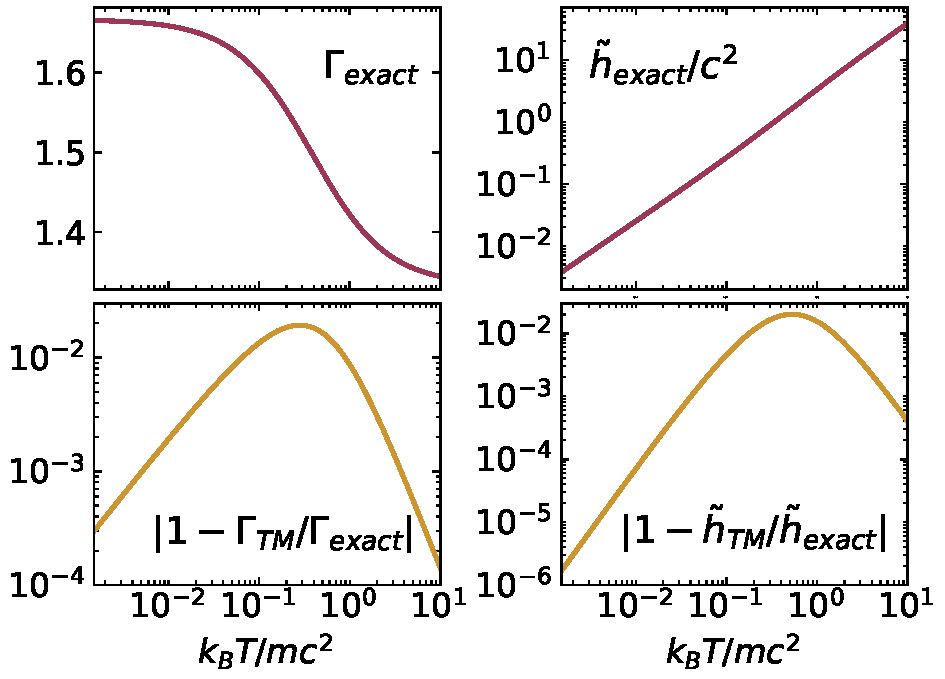
\includegraphics[width=\columnwidth]{srhd-figures/compare_eos.pdf}
    \caption{The effective adiabatic index $\Gamma$ (top left), the reduced enthalpy $\tilde{h}/c^2\coloneqq h/c^2-1$ (top right) as a function of temperature. Bottom panels show that \Cref{TM EOS} approaches \Cref{EXACT_EOS} in both high- and low-$T$ limits, where the maximum relative errors $\abs{1-\Gamma_{\text{TM}}/\Gamma_{\text{exact}}}$ and $\abs{1-\tilde{h}_{\text{TM}}/\tilde{h}_{\text{exact}}}$, are only 1.9 and 2.0 per cent, respectively.}
   \label{fig:compare_eos}
\end{figure}


\section{Conversion between primitive and conserved variables}
\label{section: Conversion between primitive variables and conserved ones}
In standard Riemann-type numerical schemes, conversion between conserved and primitive variables is a common procedure for data reconstructions and flux computations. For non-relativistic hydrodynamics, this conversion can be carried out in a straightforward and analytical manner. However, designing an accurate and efficient conversion algorithm for a relativistic problem in the presence of NR gases, which involves root-finding, is challenging. This is because catastrophic cancellations may arise in the non-relativistic gas.

Here we propose a new conversion scheme to solve this problem based on the TM EoS. The reduced energy density (Equation \ref{ETilde}) and the momentum density (Equation \ref{momentum}) satisfy the relation
\begin{equation}
\begin{aligned}
&\left(\frac{\tilde{E}}{Dc^2}\right)^2+2\left(\frac{\tilde{E}}{Dc^2}\right)-\left(\frac{\abs{\mathbf{M}}}{Dc}\right)^2
\\&= \frac{\tilde{h}^2}{c^4}+\frac{2\tilde{h}}{c^2}-2\left(\frac{k_{B}T}{mc^2}\right)\left(\frac{\tilde{h}}{c^2}+1\right)+\frac{\left(k_{B}T/mc^2\right)^2\left(\tilde{h}+c^2\right)^2}{\left(\tilde{h}+c^2\right)^2+\left(\frac{\abs{\mathbf{M}}c}{D}\right)^2}\\
&\coloneqq f\left(\tilde{h}\right),
\end{aligned}
\label{transcendental equation}
\end{equation}
where $f$ is positive definite, $\tilde{h}\coloneqq h-c^2$ is the reduced enthalpy, and the temperature $k_{B}T/mc^2$ is related to $\tilde{h}$ by inverting \Cref{TM EOS}:
\begin{equation}
\frac{k_{B}T}{mc^2}=\frac{2\left(\tilde{h}/c^2\right)^2+4\left(\tilde{h}/c^2\right)}{5\left(\tilde{h}/c^2\right)+5+\sqrt{9\left(\tilde{h}/c^2\right)^2+18\left(\tilde{h}/c^2\right)+25}}.
\label{T of h}
\end{equation}

The conserved variables ${\tilde E}$, $M^{j}$, and $D$ on the left-hand side are known quantities updated at every time step, from which one can solve for $\tilde{h}$.

We adopt $\tilde{h}=h-c^2$ instead of $h$ as the root because the latter is dominated by rest mass energy density in the low-$T$ limit and thus will suffer from catastrophic cancellation when numerically extracting temperature from trailing digits.


\Cref{transcendental equation} is suitable for the Newton-Raphson iteration method as it is a monotonically increasing function of $\tilde{h}$. That is, \Cref{transcendental equation} has no zero derivative of $\tilde{h}$ that might otherwise lead to a divergence of the iterative procedure. The Newton-Raphson method requires an initial guess of $\tilde{h}$ and the derivative of \Cref{transcendental equation} for iteration, both of which are presented in Appendix \ref{The choice of initial guesses}. We adopt the convergence criterion $\abs{1-\tilde{h}_{i}/\tilde{h}_{i+1}}\leq\epsilon_{\text{machine}}$, where $\tilde{h}_{i}$ is the approximate root at the $i$th iteration and $\epsilon_{\text{machine}}$ is the machine precision ($10^{-7}$ and $10^{-16}$ for single and double precision, respectively).

After obtaining $\tilde{h}$, we substitute it into Equation~(\ref{momentum}) to get four-velocity:
\begin{equation}
U^i=\frac{M^{i}c^2}{D\left(c^2+\tilde{h}\right)}.\label{eq:four-velocity}
\end{equation}
Next, we compute the Lorentz factor and proper mass density from Equation~(\ref{eq:new expression of Lorentz factor}) and Equation~(\ref{density}) and then use Equation~(\ref{T of h}) to obtain temperature. Finally, the pressure is given by
\begin{equation}
    p=\rho c^2 \left(\frac{k_{B}T}{mc^2}\right).
    \label{eq:p=rhoT}
\end{equation}

Justifying the superiority of our new conversion scheme using $\tilde{E}$, we estimate the relative error of computing $a-b$ by \citep{Nicholas}
\begin{equation}
\frac{\left|a\right|+\left|b\right|}{\left|a-b\right|}\epsilon_{\text{machine}}. \label{error bound of subtraction}
\end{equation}
Thus, the error of the new conversion scheme can be estimated by substituting\\
$\left[\left(\tilde{E}/Dc^2\right)^2+2\left(\tilde{E}/Dc^2\right)\right]$ and $\left(\abs{\mathbf{M}}/Dc\right)^2$ for $a$ and $b$, respectively, in \Cref{error bound of subtraction}. The error in terms of primitive variables reads
\begin{equation}
\begin{aligned}
\label{eq:ImprovedRelativeError}
&\left[\frac{\gamma^2\left(\tilde{h}+1\right)^2\left(1+\beta^2\right)+\frac{T^2}{\gamma^2}-2\left(\tilde{h}+1\right)T-1}{\left(\tilde{h}+1\right)^2+\frac{T^2}{\gamma^2}-2\left(\tilde{h}+1\right)T-1}\right]\epsilon_{\text{machine}}\\
&\approx \left(1+\mathscr{M}^2\right)\epsilon_{\text{machine}},
\end{aligned}
\end{equation}
where $\beta=\sqrt{v^{i}v_{i}}/c$. The approximate equality in \Cref{eq:ImprovedRelativeError} holds for all finite temperature.

According to \Cref{eq:MachNumber} and \Cref{eq:ImprovedRelativeError}, we can decide whether to adopt single or double precision before simulations. Taking ultra-relativistic pulsar wind ($\mathscr{M}_{\text{wind}}\approx 10^{6}$) as an example, we must use double precision to suppress the error to $10^{-4}$. But for mild-relativistic AGN jets ($\mathscr{M_{\text{jet}}} < 10$), single precision is sufficient to reduce the error to $10^{-5}$.

For the original scheme using the total energy density $E$ instead of $\tilde{E}$, a similar error estimation can be performed by replacing $\tilde{E}$ with $E-Dc^2$ on the left-hand side of \Cref{transcendental equation}, which gives
\begin{equation}
    \left[\frac{2\gamma^2\left(\tilde{h}+1\right)^2+\frac{T^2}{\gamma^2}-2\left(\tilde{h}+1\right)T+\left(\tilde{h}+1\right)^2+1}{\left(\tilde{h}+2\right)\tilde{h}+\frac{T^2}{\gamma^2}-2\left(\tilde{h}+1\right)T}\right]\epsilon_{\text{machine}}.
\label{eq:OriRelativeError}
\end{equation}

\Cref{fig:ErrorDistribution} shows the contour plots of \Cref{eq:ImprovedRelativeError} for the new scheme (top panel) and \Cref{eq:OriRelativeError} for the original scheme (middle panel) as a function of $\mathscr{M}$ and temperature. The bottom panel shows the ratio of \Cref{eq:OriRelativeError} to \Cref{eq:ImprovedRelativeError}. It demonstrates the advantage of using $\tilde{E}$. The top panel shows that using $\tilde{E}$ in the conversion scheme is almost error-free when dealing with subsonic flows at any finite temperature, including the low-$T$ limit. In supersonic flows, the numerical errors proportional to $\mathscr{M}^2$ are common and caused by finite digits of floating numbers. In comparison, the middle panel shows the error using $E$, which severely suffers from catastrophic cancellation in the low-$T$ limit even when $\mathscr{M}\ll 1$. See also \Cref{fig:ErrorAnalysis} in Appendix \ref{Appendix:Numerical error analysis}.


\begin{figure}
	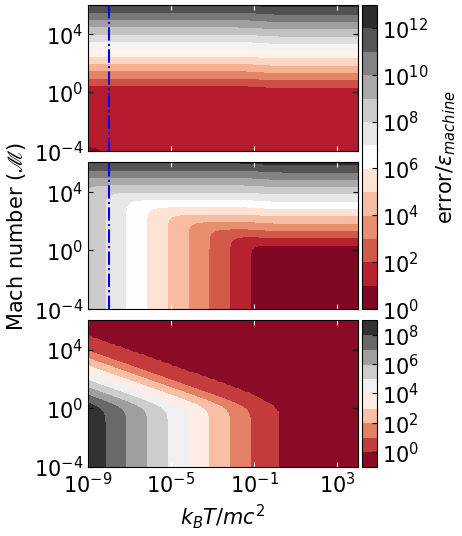
\includegraphics[width=\columnwidth]{srhd-figures/ErrorDistributionImproved.png}
    \caption{Numerical errors of the conversion from conserved to primitive variables as a function of $\mathscr{M}$ and $k_{B}T/mc^2$. The top and middle panel show the errors of the new and original schemes estimated by \Cref{eq:ImprovedRelativeError} and \Cref{eq:OriRelativeError}, respectively. The bottom panel shows the ratio of \Cref{eq:OriRelativeError} to \Cref{eq:ImprovedRelativeError}. \Cref{fig:ErrorAnalysis} in Appendix \ref{Appendix:Numerical error analysis} provides numerical evidences showing a remarkable consistency with the predicted values at $k_{B}T/mc^2=10^{-8}$ (blue dashed-dotted line).}
   \label{fig:ErrorDistribution}
\end{figure}

On the other hand, conversion from primitive to conserved variables is also needed in the Riemann solver. This procedure involves straightforward substitution without the need of root-finding. We use
\begin{equation}
\frac{\tilde{h}}{c^2} = 2.5\left(\frac{k_{B}T}{mc^2}\right)+\frac{2.25\left(k_{B}T/mc^2\right)^2}{1+\sqrt{2.25\left(k_{B}T/mc^2\right)^2+1}},
\label{eq:T_to_HTilde}
\end{equation}
and
\begin{equation}
\frac{\tilde{E}}{Dc^2} = \frac{\left(\frac{\abs{\mathbf{M}}}{Dc}\right)^2+f\left(\tilde{h}\right)}{1+\sqrt{1+\left(\frac{\abs{\mathbf{M}}}{Dc}\right)^2+f(\tilde{h})}},
\label{eq:E_D}
\end{equation}
to compute $\tilde{h}$ and $\tilde{E}$, where $f(\tilde{h})$ can be computed from \Cref{transcendental equation} with known $\abs{\mathbf{M}}/Dc$. Note that \Cref{eq:T_to_HTilde} and \Cref{eq:E_D}, following directly from \Cref{TM EOS} and \Cref{transcendental equation} without any approximation, are written in a form without any subtraction to avoid catastrophic cancellation. In contrast, using \Cref{definition of reduced energy} and \Cref{ETilde} to compute the reduced energy density $\tilde{E}$ can suffer from catastrophic cancellation in the NR limit.

We close this section by providing a flowchart of the new conversion scheme in \Cref{fig:flowchart} in Appendix \ref{Appendix:Numerical error analysis} and by summarizing the equations actually solved by \textsc{gamer-sr}. Other mathematically equivalent forms are unrecommended as they may suffer from catastrophic cancellation in the UR or NR limit.
\begin{itemize}
\item Evolution equations: Equation~(\ref{D evolution}, \ref{M evolution}, \ref{ETilde evolution}).
\item Lorentz factor:
\Cref{eq:new expression of Lorentz factor}.
\item Four-velocities: \Cref{eq:four-velocity}.
\item Temperature: \Cref{T of h}.
\item Pressure: \Cref{eq:p=rhoT}.
\item Reduced enthalpy: \Cref{eq:T_to_HTilde}.
\item Reduced energy density: \Cref{eq:E_D}.
\end{itemize}

